\section{Tools}
In this section, we will describe the tools used to create our system.

\subsection{UPPAAL}
Uppaal is a tool box for validation (via graphical simulation) and verification (via automatic model-checking) of real-time systems. The idea is to model a system using timed automata, as defined in Section \ref{sec:automate}, simulate it and then verify properties that we can define on it. Those automata will be synchronized through channels. Because Uppaal is based on timed automata, clocks will be an important thing in this software. Indeed, the time will be handle thanks to those clocks. We will see that it will be possible to test the value of a clock or even to reset it. Also, clocks will progress in the whole system at the same time.
\begin{figure}[H]\label{fig:uppaal}
  \begin{center}
    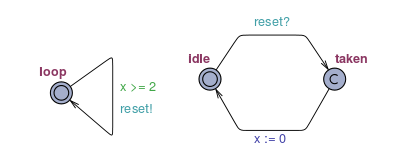
\includegraphics[width=0.8\textwidth]{picture/uppaal.png}
    \caption{Basic example made with UPPAAL}
  \end{center}
\end{figure}
 In Figure \ref{fig:uppaal}, two different elements can be seen. On the left part, there is a loop that will, when the clock x is higher or equal to 2, trigger a reset transition. On the right part, we have a system that wait for a reset. When the trigger has been done by the left component, it is send to the right component thanks to the channels between them. If the reset has been done, we transit into the taken state before going back to the Idle state and resetting the x clock to 0. This program then repeat itself.
 
\subsection{UPPAAL TiGa}
 Tiga is an extension of Uppaal, allowing timed games. The main difference with Uppaal is the possibility of having transitions taken non-deterministically by the environment. Indeed, while in UPPAAL everything is defined by the controller, in TiGa, the environment can also play. Since it is a game between the controller and the environment, we would want to find a winning strategy. In our case, as said in Section \ref{sec:game}, the controller will be the traffic lights while the environment will be the buses and the pedestrians.
 \begin{figure}[H]\label{fig:tiga}
  \begin{center}
    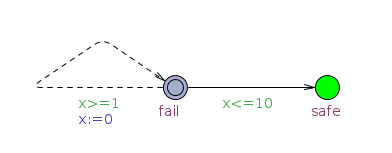
\includegraphics[width=0.8\textwidth]{picture/tiga.png}
    \caption{Basic example made with UPPAAL TiGa}
  \end{center}
\end{figure}
In this example, the environment is represented by the cut lines. We start from the fail state and two different states can be reached. Either we go back to the left state because the environment decided to take his transition and to reset the clock x to 0, either to go to the safe state if the controller decided so. If the controller and the environment want to play at the same time, the environment actually plays.
